\subsection{MessageBroker}\label{sec:mit-messageBroker}
The \lstinline|MessageBroker| is dealing with incoming messages. To do so, it is observing all opened direct connections. When a new message is received the message broker first checks whether the message is targeting the peer itself or whether the message is addressed to another peer and needs to be forwarded. The message can also have a broadcast address. In case of a broadcast address the MessageBroker is forwarding the message to all known peers with a direct connection, except for the inbound connection.

When the message has found its destination, the MessageBroker is processing the message further based on the subject.

\begin{figure}
\centering
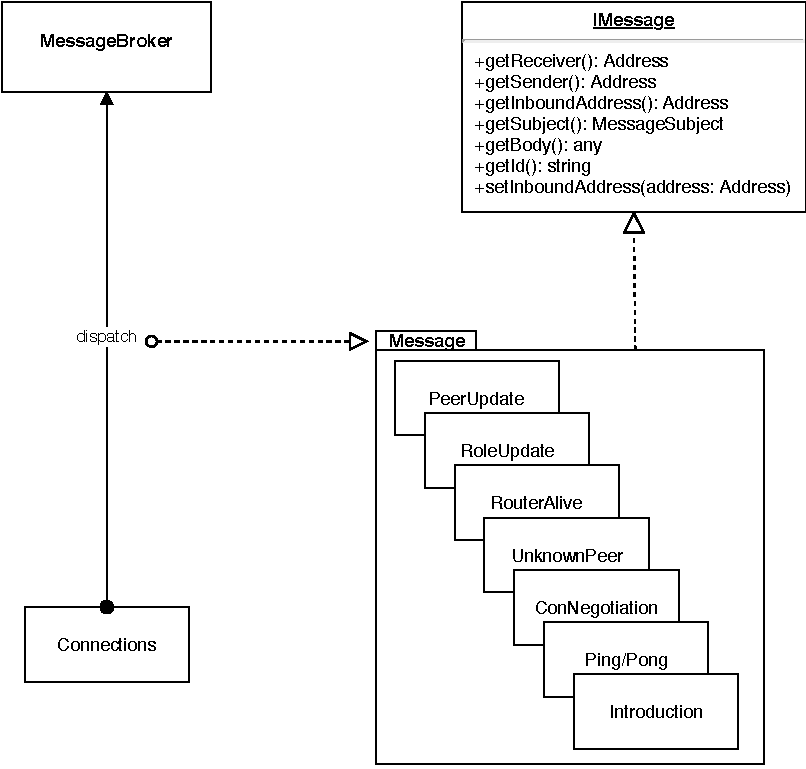
\includegraphics[width=0.75\textwidth]{graphics/implementation/mitosis-architecture-messages.pdf}
\caption{MessageBroker}
\label{fig:mit-messages}
\end{figure}

Message types are identified by the subject of a message. Available subjects are briefly described in the following.
\begin{itemize}
    \itembf{Introduction}
    \label{itm:mit-msg-introduction}
        Sent by the peer when it is contacting the \signal peer for the first time. 
        MessageBroker is not processing this message as the RoleManager is taking care of it.
    \itembf{PeerUpdate}
    \label{itm:mit-msg-PeerUpdate}
        A \peerUpdate is sent by one peer to another to let them know about its direct connections. The receiving party can then update its RemotePeer table accordingly.
        MessageBroker is delegating to the PeerManger to \lstinline|updatePeers|.
    \itembf{RoleUpdate}
    \label{itm:mit-msg-RoleUpdate}
        When a peer is promoted to a new role this is communicated via a \roleUpdate. However, only a peer with the same role or a superior role can promote a peer.
        MessageBroker is delegating to the RoleManager to \lstinline|updateRoles|.
    \itembf{ConnectionNegotiation}
    \label{itm:mit-msg-ConnectionNegotiation}
        \Glspl{connection-negotiation} have to be exchanged in order to open a WebRTC connection. Four different kind of \glspl{connection-negotiation} are available: \lstinline|request|, \lstinline|offer|, \lstinline|answer|, \lstinline|reject|.
        MessageBroker is delegating to the PeerManager to \lstinline|negotiateConnection|.
    \itembf{RouterAlive}
    \label{itm:mit-msg-RouterAlive}
        A peer with the \routerRole role is broadcasting \routerAlive messages continuously to let other peers in the cluster know that it still exists.
        MessageBroker is flooding this message to all direct peers, unless it has already flooded a \routerAlive for the given sequence number and delegates it to PeerManager to \lstinline|handleRouterAlive|.
    \itembf{UnknownPeer}
    \label{itm:mit-msg-UnknownPeer}
        \Gls{unknown-peer} is sent to all direct peers when a RemotePeer is removed from the RemotePeer table. Other peers can update their RemotePeer table accordingly.
        MessageBroker is delegating to the PeerManager who then closes all connections for the given RemotePeer address.
    \itembf{Ping/Pong}
    \label{itm:mit-msg-PingPong}
        \Gls{ping-pong} messages are exchanged by the WebRTC data connection to measure the transmission quality (\vref{par:webrtc-data-measure-quality}).
        MessageBroker is not further processing \glspl{ping-pong}.
    \itembf{ChannelAnnouncement}
    \label{itm:mit-msg-ChannelAnnouncement}
        \Gls{channel-announcement} messages are dispatched by a peer when it has an active provider for a broadcast channel (\vref{chap:mitosis-stream}).
        MessageBroker is delegating to the ChannelManager to \lstinline|updateProviders|.
\end{itemize}
